
\subsection{Simulated Annealing}


\textit{Simulated annealing} is a metaheuristic optimization technique inspired by the annealing process in metallurgy, where metals are cooled gradually to achieve a stable state with minimized energy \citep{kirkpatrick1983optimization}. In the context of keyboard optimization, it is used as an iterative algorithm that explores different keyboard layouts by gradually accepting key swaps that reduce the overall energy (i.e., predicted typing time). Unlike gradient descent and other methods that always aim for an absolute minimum, simulated annealing allows for the occasional acceptance of higher-cost solutions to explore a broader search space, preventing the algorithm from getting stuck in local optima. Eventually, simulated annealing converges toward a stable, low-cost configuration -- the global minimum or an approximation of it. 

% A key challenge in applying simulated annealing effectively lies in selecting appropriate parameters that govern the algorithm's behavior, including the initial temperature and the termination criterion. These parameters can significantly influence the algorithm's convergence and the quality of the solution obtained. Traditionally, parameter selection has relied on manual estimation based on domain knowledge and experimentation, which can be time-consuming and may not generalize well across different problem instances \citep{Ben-Ameur2004}. To address this, this paper outlines a dynamic approach to setting the initial temperature and termination criterion, allowing for greater flexibility and adaptability when exploring layouts under various data modifications. For example, analyzing layouts at different WPM ranges, optimizing for specific subsets of keys, or using different corpora can lead to substantial variations in the cost function and the number of swaps required for convergence. The dynamic parameter setting approach ensures that the simulated annealing algorithm can effectively explore the solution space and converge towards an optimal layout, regardless of these variations.


Selecting the parameters in simulated annealing for convergence can be challenging, usually requiring experimentation or domain knowledge \citep{SAOverview}. We outline a dynamic approach to setting the initial temperature and termination criterion to address this. This ensures layouts can be explored across a variety of data modifications. For example, layouts may be optimized for different WPM ranges, languages, or a specific subset of keys. In these cases, the cost function may yield drastically different values, and the number of swaps required for convergence may vary, necessitating adjustments to the parameters.

% Proofs of the simulated annealing's effectiveness are outside of the scope of this paper.
\subsubsection{Solution Space and Transitions}
\noindent A crucial step in implementing simulated annealing is defining the solution space and transition process. This allows the algorithm to explore potential solutions effectively. Changes to the solution should occur gradually to ensure smooth traversal of the solution landscape, preventing abrupt jumps that overlook promising solutions \citep{SAOverview}.

For keyboard optimization, a solution is defined as a mapping between characters and their positions on a matrix, as illustrated in Table ~\ref{fig:keyboard_matrix}. The chosen coordinate system mirrors real-world keyboard usage by grouping fingers based on absolute values, differentiating hands by sign, and enabling easy distance calculations. This encoding strategy allows the algorithm to effectively evaluate the ergonomic implications of different key arrangements. A transition is defined as the swapping of two keys on the keyboard matrix. % Consequently, the neighborhood of a given layout consists of all layouts that can be generated as the result of a single key pair swap.

The acceptance of candidate solutions in simulated annealing is determined by a probabilistic criterion derived from the Boltzmann distribution function. Originating from statistical mechanics, this function describes the probability of particles occupying different energy states within a system \citep{harris2004introduction}. This criterion is mathematically represented as follows:

\begin{equation*}
A(i) = 
\left\{ 
\begin{array}{lr}
    \exp \left( -\frac{\Delta E}{T} \right), & \text{if } \Delta E > 0 \\
    1, & \text{otherwise}
\end{array}
\right.
\end{equation*}

\noindent Here, $\Delta E$ represents the change in energy within the system or, in this case, in the estimated typing time between the current layout and the candidate layout, and $T$ denotes the temperature, a parameter that controls the amount of randomness in the system. If the change in typing time is negative ($\Delta E < 0$), indicating an improvement in estimated typing time, the candidate layout is accepted with certainty. However, if the change in estimated typing time is positive, indicating a worsening layout, the candidate layout is accepted with a probability determined by the Boltzmann factor, which is more likely to accept slight decreases in performance over larger ones.

This choice of probabilistic criterion allows the simulated annealing algorithm to converge on an optimal or near-optimal solution through gradual refinement \citep{granville1994simulated}. Initially, the temperature is high, allowing the algorithm to explore the solution space and escape local minima by accepting suboptimal moves. As the algorithm progresses and the temperature decreases, the probability of accepting suboptimal moves diminishes, refining the search to more promising regions. The reduction in temperature is controlled by a cooling schedule, which dictates how fast and effectively the algorithm converges to a solution. We adopt a monotonically decreasing geometric cooling schedule defined as follows:
\begin{equation*}
T_i = \alpha^i T_0
\end{equation*}

\noindent where $T_0$ is the initial-temperature and $a$ is the cooling-rate, $0 < a < 1$.

\begin{figure}[h]
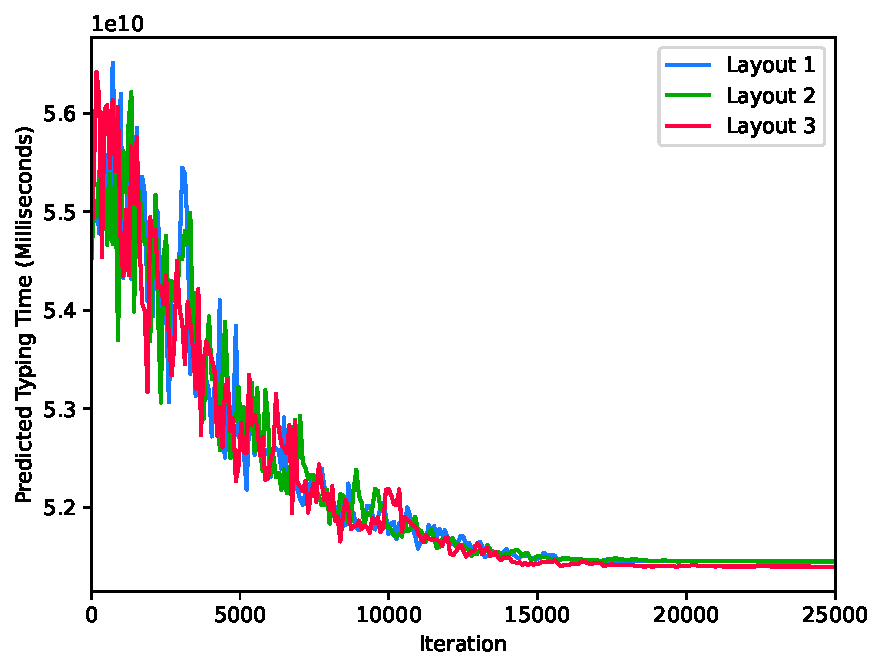
\includegraphics[width=\columnwidth]{figures/convergence.pdf}
\caption{Convergence of Estimated Typing Time during Simulated Annealing}
\label{fig:bigram_typing_time}
\end{figure}



\subsubsection{Setting the Initial Temperature}
\noindent Before any transitions are performed, an initial temperature must be set for the cooling schedule to iterate on. A common approach to setting the initial temperature is to manually estimate it based on the problem domain and its characteristics. This initial temperature is frequently chosen so that the acceptance probability at the beginning of simulated annealing is approximately equal to some value. Lacking relevant literature for our problem domain, we resort to the approach outlined in  ~\citet{Ben-Ameur2004}. We set a variable $\chi_0$ to be the desired initial acceptance probability of suboptimal transitions at the beginning of the algorithm. An iterative method is employed to compute the initial temperature $T_0$ such that the acceptance probability approaches $\chi_0$. To compute the estimated acceptance probability $\hat{\chi}(T)$ for a given temperature $T$, first, we use the set $S$ of possible positive transitions (i.e., transitions where $E_{before} < E_{after}$), where each transition $s$ represents a swap of two keys. Finally, we take the ratio between the sum of probabilities of generating and accepting each positive transition $s$ and the sum of the probabilities of generating each positive transition $s$:
\begin{equation*}
\hat{\chi}(T_n) = \frac{
    \sum_{s \in S} \exp \left( -\frac{E_{after}(s)}{T_n} \right)}
    {\sum_{s \in S} \exp \left( -\frac{E_{before}(s)}{T_n} \right)}
\end{equation*}
This can now be used to find $T_0$. First, we define an initial guess temperature $T_1$, then recursively apply this formula:
\begin{equation*}
T_{n+1} = T_n \left(\frac{\ln(\hat{\chi}(T_n))}{\ln{(\chi_0)}} \right)
\end{equation*}
Once $|\hat{\chi}(T_n) - \chi_0| \leq \epsilon$ for some error $\epsilon$, we have found our initial temperature $T_0$. 

\subsubsection{Termination Criterion}
\noindent Finally, we establish a termination criterion for the simulated annealing process to be the point at which the number of iterations lacking improvement reaches the probabilistic threshold that all potential swaps have been evaluated. We do this to ensure the simulated annealing algorithm has settled on some minima while allowing suboptimal swaps to be heuristically accepted, potentially escaping local minima.

To find the termination criterion, let $S$ be the number of iterations to evaluate all potential swaps. Let $k$ be the number of keys; for $k$ keys, the number of swappable key pairs $n = \binom{k}{2}$. We consider $S = \sum_{i=1}^{n} s_i$ where $s_i$ is the number of iterations required to evaluate the $i$-th pair after $i-1$ pairs have been evaluated.

The probability $P_i$ of selecting a new pair to swap is $P_i = \frac{n-(i-1)}{n} = \frac{n-i+1}{n}$. Consequently, $s_i$ follows a geometric distribution with an expectation of $\text{E}(s_i) = \frac{n}{n-i+1}$.

\noindent By the linearity of expectations, we derive:
\begin{align*}
\text{E}(S) = n \sum_{i=1}^{n} \frac{1}{i}
\end{align*}
To increase performance, we can use the approximation:
\begin{align*}
\text{E}(S) = n \log{n} + \gamma n + \frac{1}{2} +  O\left(\frac{1}{n}\right)
\end{align*}
where $\gamma \approx 0.5772156649$ is the Euler-Mascheroni constant. Since the number of iterations must be a positive integer, we set our final stopping point to be:
\begin{align*}
\left\lceil \binom{k}{2} \log{\binom{k}{2}} + \gamma \binom{k}{2} + \frac{1}{2} \right\rceil
\end{align*}


% \noindent The layout produced in this paper optimizes for the main block of 30 keys. So the number of possible swaps is $\binom{30}{2} = 435$ resulting in a stopping point of $\left\lceil \binom{30}{2} \log{\binom{30}{2}} + \gamma \binom{30}{2} + \frac{1}{2} \right\rceil = 2,895$ iterations.

% Manual newpage inserted to improve layout of sample file - not
% needed in general before appendices/bibliography.